\subsection{Graphit}
Die Graphitschicht konnte magnetisch auf der Probenhalterung angebracht werden. Die Vorbereitungen f�r die Graphitmessung dauerten nicht lange, da nach wenigen Versuchen eine funktionsf�hige Pt-Ir-Spitze angefertigt werden konnte. F�r die Anfertigung der Pt-Ir-Spitze standen Isopropanol, Reinigungst�cher, eine Pinzette und geeignete Zangen zum anspitzen und halten des Pt-Ir-Drahtes zu Verf�gung.
\subsubsection{Rauheit}
\begin{figure}[H]
\centering
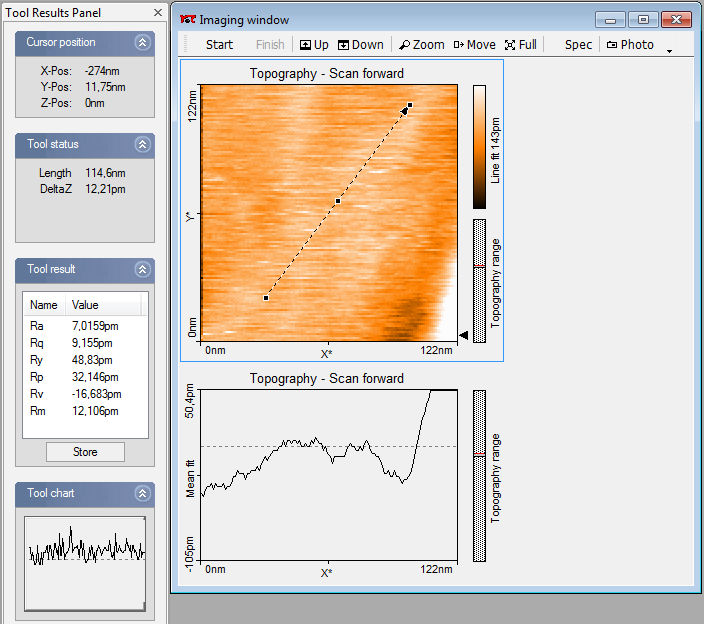
\includegraphics[scale = 0.75]{snipping_122_linienrauheit}
\caption{ Mittlere Linienrauheit von Graphit ($R_a = \SI{7,0159}{pm}$ und $R_q = \SI{9,155}{pm}$) }
\end{figure}
\begin{figure}[H]
\centering
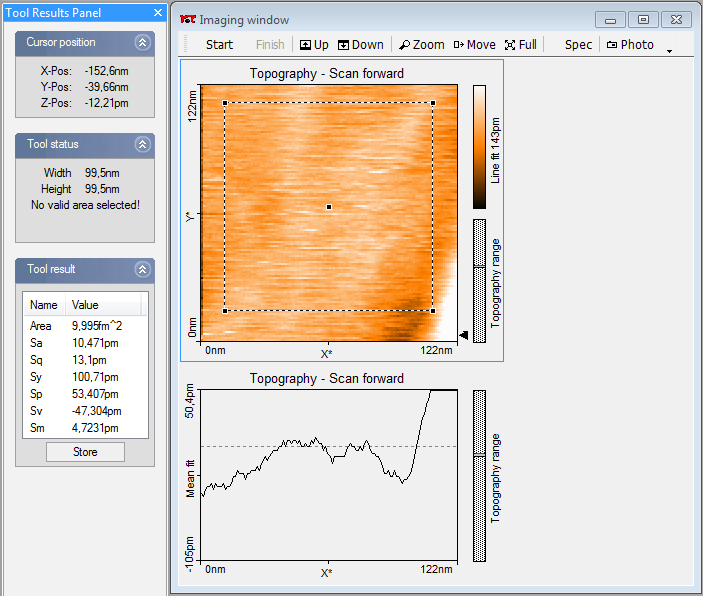
\includegraphics[scale = 0.75]{snipping_122_flaechenrauheit}
\caption{ Mittlere Fl�chenrauheit von Graphit ($S_a = \SI{10,471}{pm}$ und $S_q = \SI{13,1}{pm}$) }
\end{figure}
\subsubsection{Gitterstruktur und Elektronendichteverteilung}
\subsubsection{Mittlerer Atomabstand}